\chapter{Estado del Arte}\label{chapter:state-of-the-art}

\section{Introduccion de RL}\label{section:state-of-the-art:introduction-to-RL}

La idea de aprender interactuando con el entorno es probablemente lo primero que se piensa cuando se habla en la naturaleza del aprendizaje. Cuando un bebé juega, agita los brazos o mira a su alrededor, no tiene un maestro explícito, pero sí una conexión sensoriomotora directa con su entorno. El ejercicio de esta conexión produce una gran cantidad de información sobre la causa y el efecto, sobre las consecuencias de las acciones y sobre lo que hay que hacer para alcanzar los objetivos. A lo largo de su vida, estas interacciones son, sin duda, una importante fuente de conocimiento sobre el entorno y sobre ellos mismos. Tanto si aprenden a conducir un coche como a mantener una conversación, son muy consciente de cómo responde el entorno a lo que hacen, y tratan de influir en lo que ocurre a través de su comportamiento. El aprendizaje a partir de la interacción es una idea fundamental que subyace en casi todas las teorías del aprendizaje y la inteligencia y cualquier método que se adapte bien a la resolución de este tipo de problemas lo consideramos un método de aprendizaje por refuerzo.


En inteligencia artificial la tarea básica del aprendizaje por refuerzo consiste en capturar los aspectos más importantes del problema al que se enfrenta un agente que interactúa con su entorno para lograr un objetivo. Está claro que un agente de este tipo debe ser capaz de percibir el estado del entorno hasta cierto punto y debe ser capaz de realizar acciones que afecten al estado. El agente también debe tener uno o varios objetivos relacionados con el estado del entorno. Los problemas de aprendizaje por refuerzo implican aprender qué hacer, o sea cómo asignar situaciones a acciones, para maximizar una señal de recompensa numérica. En esencia, se trata de problemas de bucle cerrado porque las acciones del sistema de aprendizaje influyen en sus entradas posteriores. Además, no se le dice al agente qué acciones debe tomar, como en muchas formas de aprendizaje automático, sino que debe descubrir qué acciones producen la mayor recompensa al probarlas [Fig. \ref{fig:rl-elements}]. En los casos más interesantes y desafiantes, las acciones pueden afectar no sólo a la recompensa inmediata, sino también a la siguiente situación y, a través de ella, a todas las recompensas posteriores.

\begin{figure}[ht!]
    \centering
    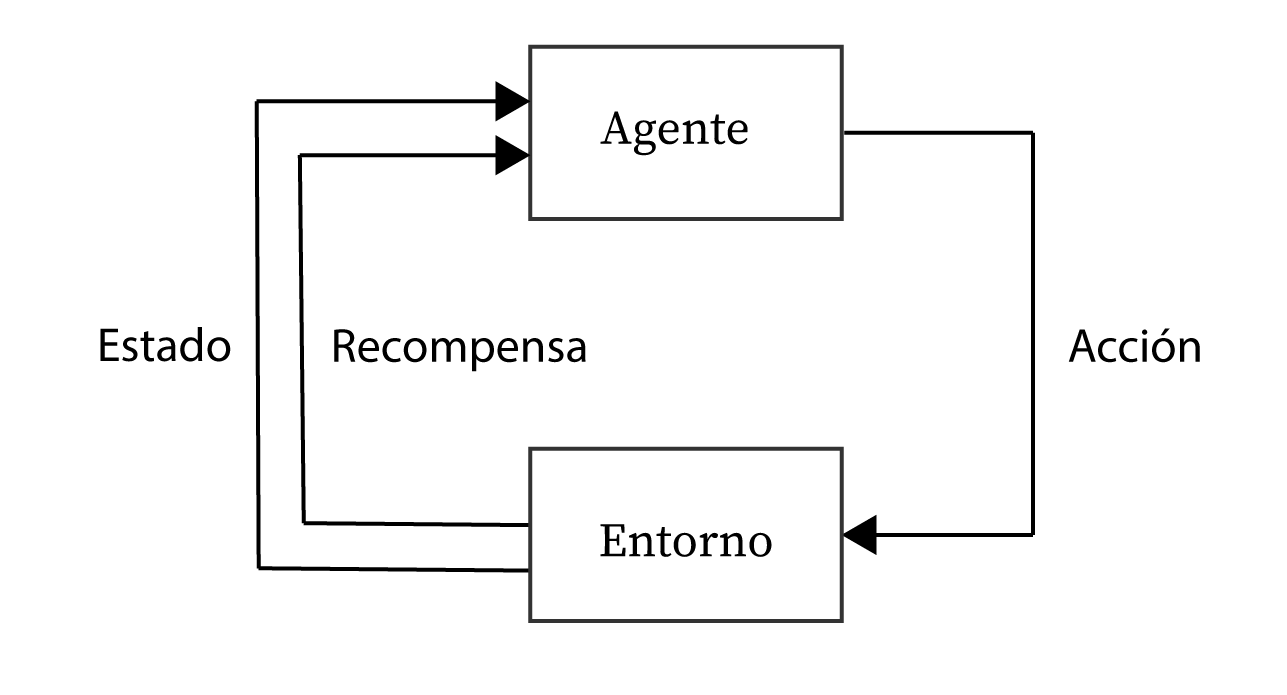
\includegraphics[width=0.7\textwidth]{Graphics/rl-elements.png}
    \caption{Diagrama de los componentes elementales del aprendizaje por refuerzo.}
    \label{fig:rl-elements}
\end{figure}

\subsection*{Componentes del aprendizaje por refuerzo}

Más allá de los macroconceptos de agente, entorno, observaciones y acciones, se pueden identificar cuatro subelementos principales de un sistema de aprendizaje por refuerzo: la política, la señal de recompensa, la función de valor y, opcionalmente, el modelo del entorno.

La política define la forma de actuar del agente en un momento dado. A grandes rasgos, una política es un mapeo de los estados percibidos del entorno a las acciones que se deben realizar cuando se encuentran en esos estados. La política es el núcleo de la voluntad de un agente en el sentido de que por sí sola es suficiente para determinar su comportamiento. En general, las políticas pueden ser estocásticas.

La señal de recompensa define el objetivo en un problema de aprendizaje por refuerzo. En cada paso de tiempo, el entorno envía al agente de aprendizaje por refuerzo un único número, una recompensa. El único objetivo del agente es maximizar la recompensa total que recibe a largo plazo. La señal de recompensa define, pues, cuáles son los eventos buenos y malos para el agente. La recompensa enviada en cualquier momento depende de la acción del agente y el estado actual del entorno. El agente no puede alterar el proceso que lo hace. La única forma en que el agente puede influir en la señal de recompensa es a través de sus acciones, que pueden tener un efecto directo en la recompensa, o un efecto indirecto a través del cambio del estado del entorno.

Las recompensas son en cierto modo primarias, mientras que los valores, como predicciones de las recompensas, son secundarios. Sin recompensas no podría haber valores, y el único propósito de estimar los valores es conseguir más recompensas. Sin embargo, son los valores los que más nos preocupan a la hora de tomar y evaluar decisiones. Las elecciones de acción se hacen en base a juicios de valor. Buscamos acciones que provoquen estados de mayor valor, no de mayor recompensa, porque estas acciones obtienen la mayor cantidad de recompensa para nosotros a largo plazo. En la toma de decisiones y la planificación, la cantidad derivada llamada valor es la que más nos preocupa. Por desgracia, es mucho más difícil determinar los valores que las recompensas. Las recompensas vienen dadas directamente por el entorno, pero los valores deben estimarse y reestimarse a partir de las secuencias de observaciones que realiza un agente a lo largo de su vida. De hecho, el componente más importante de casi todos los algoritmos de aprendizaje por refuerzo que consideramos es un método para estimar eficazmente los valores.

El cuarto y último elemento de algunos sistemas de aprendizaje por refuerzo es un modelo del entorno. Se trata de algo que imita el comportamiento del entorno o, más generalmente, que permite hacer inferencias sobre cómo se comportará el entorno. Por ejemplo, dado un estado y una acción, el modelo puede predecir el siguiente estado y la siguiente recompensa resultantes.


\subsection*{Proceso de Decisión de Markov (MDP)}

Idealmente, es una señal de estado que resuma las sensaciones pasadas de forma compacta, pero de tal manera que se conserve toda la información relevante. Esto requiere normalmente más que las sensaciones inmediatas, pero nunca más que la historia completa de todas las sensaciones pasadas. Una señal de estado que consigue retener toda la información relevante se dice que es Markov, o que tiene la propiedad Markov.

Siempre queremos que el estado sea una buena base para predecir futuras recompensas y para seleccionar acciones. Los estados de Markov proporcionan una base insuperable para hacer todas estas cosas. En la medida en que el estado se acerque a la capacidad de los estados de Markov en estos aspectos, se obtendrá un mejor rendimiento de los sistemas de aprendizaje por refuerzo.

Una tarea de aprendizaje por refuerzo que satisface la propiedad de Markov se denomina Proceso de Decisión de Markov, o MDP. Si los espacios de estado y acción son finitos, se denomina Proceso de Decisión de Markov finito (MDP finito).

La interacción agente-entorno se descompone naturalmente en una secuencia de episodios separados (tareas episódicas), y otra en la que no (tareas continuas). El primer caso es matemáticamente más fácil porque cada acción afecta sólo al número finito de recompensas recibidas posteriormente durante el episodio.

\subsection*{Principales estrategias para resolver problemas de aprendizaje por refuerzo}

El objetivo de la RL es que el agente aprenda a navegar por el entorno para maximizar una métrica de recompensa acumulada. La política es como el algoritmo que el agente perfecciona para maximizar la recompensa. Por tanto el objetivo de la RL es construir la política que máximice la recompensa acumulada, al menos de forma implícita.

Los algoritmos de RL se pueden dividir utilizando varias categorizaciones, una de ellas está dada en el uso del modelo del entorno: los \textit{basados en modelos} y los \textit{libres de modelo}.

\begin{itemize}
\item Los \textit{basados en el modelo}, tal y como suena, tienen un agente que intenta comprender su entorno y crear un modelo para él basado en sus interacciones con este entorno. En un sistema de este tipo, las preferencias tienen prioridad sobre las consecuencias de las acciones, es decir, el agente codicioso siempre intentará realizar una acción que le permita obtener la máxima recompensa, independientemente de lo que esa acción pueda causar. Algoritmos como \textit{Dyna} son un ejemplo.

\item Por otro lado, como muestra la [Fig. \ref{fig:rl-strategies}], los algoritmos \textit{libres de modelo} buscan aprender las consecuencias de sus acciones a través de la experiencia. En otras palabras, un algoritmo de este tipo llevará a cabo una acción varias veces y ajustará la política (la estrategia que subyace a sus acciones) para obtener recompensas óptimas, basándose en los resultados.
\end{itemize}

Si el agente puede predecir (o simular) la recompensa de una acción antes de llevarla a cabo y, por tanto, planificar lo que debe hacer, el algoritmo está basado en un modelo. Mientras que si tiene que llevar a cabo la acción, o sea una experiencia real, para ver lo que ocurre y aprender de ello, no tiene modelo.

\begin{figure}[ht!]
    \centering
    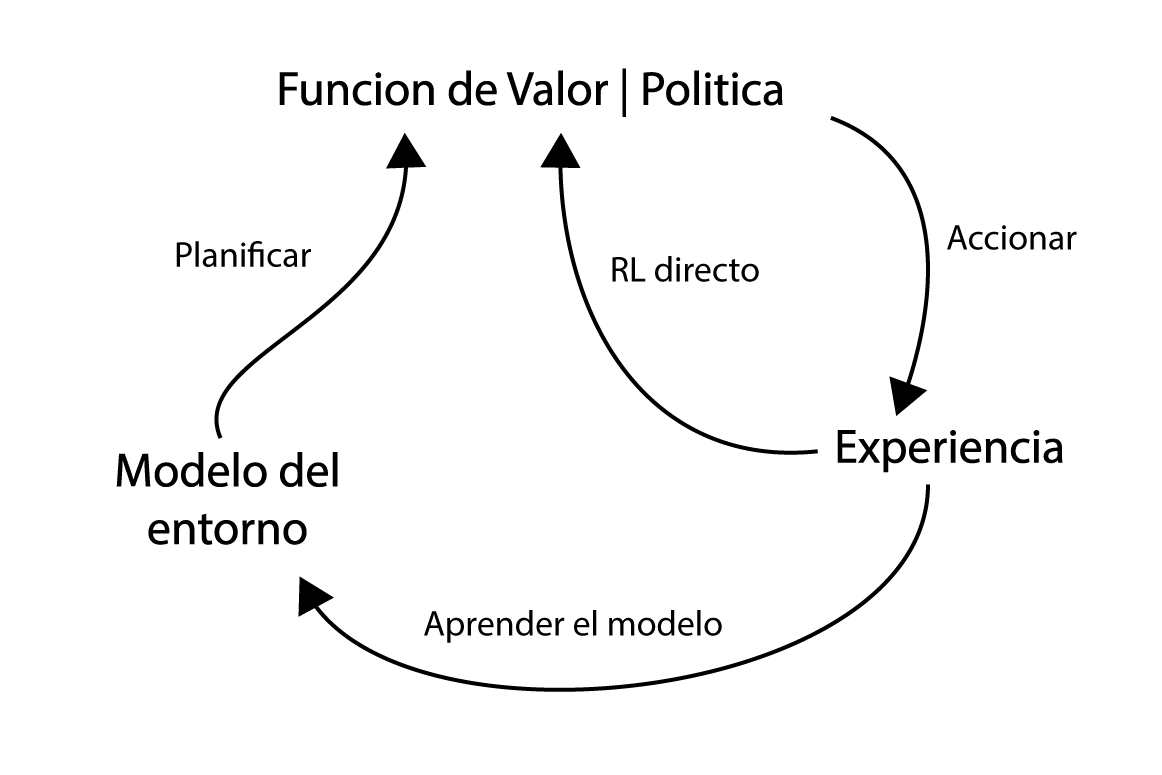
\includegraphics[width=0.7\textwidth]{Graphics/rl-strategies.png}
    \caption{Relaciones entre el aprendizaje, la planificación y la actuación.}
    \label{fig:rl-strategies}
\end{figure}


Dentro de los algoritmos  \textit{libres de modelo} existe otra caracterización basada en si se construye explicitamente o no la política del agente.

\begin{itemize}
\item En los métodos \textit{basados en políticas} se construye explícitamente una representación de una política y se mantiene en memoria durante el aprendizaje. Se puede citar los algoritmos de \textit{Policy Gradient}, \textit{Monte Carlos Tree Search}, entre otros.

\item En los métodos \textit{basados en valores} no se almancena ninguna política explícita, sólo una función de valor. La política es aquí implícita y puede derivarse directamente de la función de valor (elegir la acción con el mejor valor). Se puede citar los algoritmos de \textit{Q-Learning}, \textit{Deep Q-Learning}, \textit{SARSA}, entre otros.

\item Los algoritmos de \textit{Actor-crítico} tienen una mezcla de los dos anteriores. Se puede citar algoritmos como AlphaZero.
\end{itemize}

Los métodos on-policy intentan evaluar o mejorar la política que se utiliza para tomar las decisiones, mientras que los métodos off-policy evalúan o mejoran una política diferente a la utilizada para generar los datos. En el primer caso, el agente aprende la función de valor de la política que sigue en ese momento, mientras que en el segundo caso aprende la función de valor de la política que considera mejor en ese momento. Estas dos políticas suelen ser diferentes debido a la necesidad de explorar.

Existen muchos otros tipos de algoritmos de aprendizaje por reforzamiento, como los geneticos o evolutivos, por imitación, entre otros. Por la simplicidad del documento se omitirá sus descripciones.

\section{Generalizacion en machine learning}\label{section:state-of-the-art:generalization-on-machine-learning}

La generalización es la capacidad de manejar situaciones (o tareas) que difieren de las situaciones anteriores. En inteligencia artificial se caracteriza como el rendimiento de un modelo en entradas que no formaban parte de sus datos de entrenamiento.

La capacidad generalización se basa fundamentalmente en las nociones relacionadas a la novedad e incertidumbre. Un sistema sólo puede generalizar ante información nueva que no pueda ser conocida de antemano ni por el sistema o por su creador. Dicha capacidad puede se pone en evidencia a medida que aumenta el dominio de las tareas y problemas que se pueden manejar. Para entender mejor estas nociones se definirán varios conceptos a continuación.

\subsection*{Tipos de Generalizacion}

\begin{itemize}
\item Generalización centrada en el sistema: es la capacidad de un sistema de aprendizaje para manejar situaciones que no ha encontrado antes. La noción formal de error de generalización en la teoría del aprendizaje estadístico pertenecería aquí.

\item Generalización consciente del desarrollador: es la capacidad de un sistema, ya sea de aprendizaje o estático, para manejar situaciones que ni el sistema ni el desarrollador del sistema han encontrado antes.
\end{itemize}
\subsection*{Grados de Generalizacion}

Aunque los límites entre los grados de la escala de generalización son mayormente difusos y continuos, se ha agrupado en 4 niveles fundamentales de interés para el estudio:

\begin{itemize}
\item \textit{Ausencia de generalización:} Los sistemas de IA en los que no hay incertidumbre no muestran generalización. Por ejemplo, no se puede decir que un programa que juega a "4 en Línea" mediante una iteración exhaustiva "generalice" a todas las configuraciones del tablero.

\item \textit{Generalización local o robustez:} Es la capacidad de un sistema para manejar nuevos puntos de una distribución conocida para una sola tarea o un conjunto bien delimitado de tareas conocidas, dado un muestreo suficientemente denso de ejemplos de la distribución (por ejemplo, la tolerancia a las perturbaciones previstas dentro de un contexto fijo). Por ejemplo, se puede decir que un clasificador de imágenes que puede distinguir imágenes RGB de 150x150 no vistas anteriormente que contienen gatos de las que contienen perros, después de haber sido entrenado con muchas de esas imágenes etiquetadas, realiza una generalización local. 

\item \textit{Generalización amplia o flexibilidad:} Es la capacidad de un sistema para manejar una amplia categoría de tareas y entornos sin más intervención humana. Esto incluye la capacidad de manejar situaciones que no podrían haber sido previstas por los creadores del sistema. Podría considerarse que refleja la capacidad del ser humano en un único y amplio ámbito de actividad (por ejemplo, las tareas domésticas o la conducción en el mundo real).

\item \textit{Generalización extrema:} Describe los sistemas abiertos con la capacidad de abordar tareas completamente nuevas que sólo comparten puntos comunes abstractos con situaciones previamente encontradas, aplicables a cualquier tarea y dominio dentro de un amplio alcance. Esto podría caracterizarse como "adaptación a incógnitas desconocidas en una gama desconocida de tareas y dominios". Las formas biológicas de inteligencia (los humanos y posiblemente otras especies in- telligentes) son el único ejemplo de un sistema de este tipo en este momento.
\end{itemize}

A esta lista podríamos, en teoría, añadir una entrada más: \textit{La universalidad}, que extendería la generalidad" más allá del ámbito de las tareas relevantes para los humanos, a cualquier tarea que pueda ser abordada de forma práctica dentro de nuestro universo (nótese que esto es diferente de cualquier tarea en absoluto, tal y como se entiende en los supuestos del teorema \textit{No Free Lunch}).

Es importante destacar que el espectro de la generalización descrito anteriormente parece reflejar la organización de las capacidades cognitivas de los seres humanos tal y como se establece en las teorías de la estructura de la inteligencia en la psicología cognitiva donde se define el \textit{factor g} como una razón global y presente en el nivel de inteligencia del hombre. 

\begin{figure}[ht!]
    \centering
    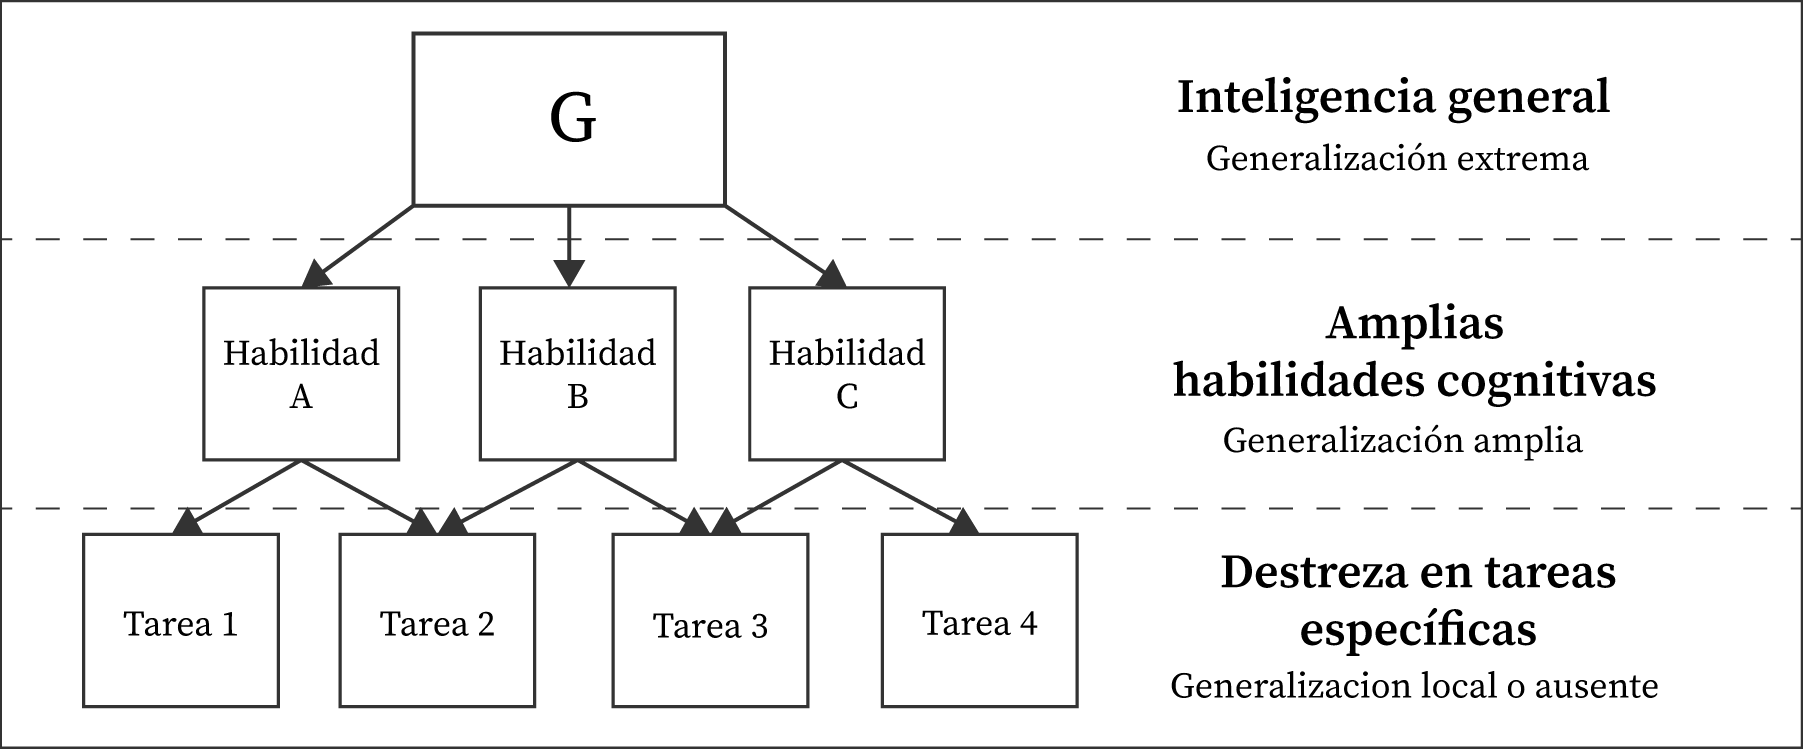
\includegraphics[width=0.7\textwidth]{Graphics/g-factor.png}
    \caption{Modelo jerárquico de las capacidades cognitivas y su correspondencia con el espectro de la generalización.}
    \label{fig:g-factor}
\end{figure}

[OUTLINE]
El objetivo de este documento son los sistemas que desarrollan capacidades extremas de generalizacion o habilidades cognitivas generales.

[OUTLINE]
Capacidad de **Generalizacion** en los algoritmos de RL. El problema de overfitting en el entrenamiento.

\section{Evaluación de algoritmos}\label{section:state-of-the-art:evaluating-algoritms}

Las medidas de rendimiento que cuantifican la habilidad de un sistema en una tarea determinada han impulsado el exito de la inteligencia artificial. No existe una forma única y formalizada de realizar una evaluación basada en la destreza. Entre los enfoques que han tenido éxito históricamente se encuentran:

\begin{itemize}
\item Revision humana: hacer que jueces humanos observen la respuesta de entrada- salida del sistema y la puntúen. Esta es la idea que subyace al test de Turing y sus variantes. Este modo de evaluación rara vez se utiliza en la práctica, debido a que es caro, imposible de automatizar y subjetivo. Algunos sistemas de IA orientados al ser humano (en particular los chatbots comerciales) lo utilizan como uno de los múltiples mecanismos de evaluación

\item Analisis en Caja-Blanca (White-Box Analysis): inspeccionar la implementación del sistema para determinar su respuesta de entrada-salida y puntuarla. Esto es más relevante para los algoritmos que resuelven una tarea totalmente descrita en un entorno totalmente descrito en el que todas las entradas posibles pueden enumerarse explícitamente o describirse analíticamente y a menudo tomaría la forma de una prueba de optimalidad.

\item Oponencial (Peer Confrontation): hacer que el sistema compita contra otras IAs o contra humanos. Este es el modo de evaluación preferido para los juegos de jugador contra jugador, como el ajedrez.

\item Comparaciones (Benchmarks): hacer que el sistema produzca resultados para un conjunto de pruebas de entradas (o entornos) para los que se conoce el resultado deseado, y puntuar la respuesta.
\end{itemize}

Particularmente los Benchmarks han aportado mucho mas. 

\section{Una buena evaluacion de Inteligencia}\label{section:state-of-the-art:a-good-measure-of-inteligence}

La base de la inteligencia. Los prejuicios y las experiencias.

Tipos de prejuicios y experiencias a considerar:
- **Premisas de bajo nivel**: Conocimientos sobre nuestro propio espacio sensoriomotor. Reflejos e instintos inatos.
- **Premisas de metaaprendizaje**: Rigen nuestras estrategias de aprendizaje y capacidades de adquisición de conocimientos.
- **Conocimientos previos de alto nivel**: Conocimientos sobre los objetos y fenómenos de nuestro entorno externo.

Las premisas de metraaprendizaje son objetivo de esta ciencia. Es la inteligencia en si misma. Entender como el cerebro transforma experiencias en conocimientos y habilidades.

La comparación entre dos sistemas debe ser JUSTA teniendo en cuenta los **Conocimientos previos de alto nivel** que posean. (remitir al problema de overfitting mencioado antes)

Tambien debe considerarse el **Ambito de tareas compartido** entre los sistemas a comparar. Y el grado de especializacion que son alcanzables en ese ambito.

Caracteristicas necesarias para una evaluacion de inteligencia extrema:
- Debe describir el Ambito de la evaluacion
- Replicable o Repoducible.
- No debe limitase a la habilidad en una tarea.
- Debe contener tareas no conocidas por los desarrolladores.
- Controlar la cantidad de experiencia que se brinda.
- Definir el conjunto de premisas de Conocimiento previo.
- Deberia funcionar para humanos y maquinas.
- Debe justificar la dificultad de generalizacion

\section{Entornos de evaluacion de Inteligencia}\label{section:state-of-the-art:inteligence-evaluation-enviroments}

Primeras pruebas propuestas

Las primeras ideas para evaluacion eran por Revision humana y tenian un caracter Antropocéntrico.

- **Juego de Imitación** (Test de Turing), explicacion.

- **Prueba del Café**, explicacion.

- **Pruebas psicometricas**, explicacion.

Comentar sobre la inefectividad y los problemas que trae hacer evaluaciones con supervision. (Mencionar las buenas practicas para evaluaciones de mas adelante)

Otas propuestas de evaluación

La actual tendencia de investigadores por desarrollar algoritmos de proposito general.  

Ejemplos de algunas evaluaciones mas modernas pero no se implementaron.

- **The bica cognitive decathlon** (2004)

- **Olimpiadas de Turing** (2014)

State of the Art

La inteligencia como capacidad de adaptacion a nuevos entornos.


\subsection{Entornos de evaluación con tareas conocidas}\label{section:state-of-the-art:inteligence-evaluation-enviroments:evaluation-enviroments-with-know-tasks}

Por lo general utilizan amplias baterías de tareas de prueba para evaluar sistemas que buscan una mayor flexibilidad. En estos entornos los desarrolladores del sistema evaluado conocen de antemano el tipo de tareas que enfrentarán, solo que los escenarios varian tantos que resolver dichas tareas requerirán diferentes formas de "razonamiento" y "creatividad", expresion directa de la generalización a partir de su entrenamiento.

La lógica subyacente de estos esfuerzos es medir algo más general que la habilidad en una tarea específica ampliando el conjunto de tareas objetivo. Sin embargo, cuando se trata de evaluar la flexibilidad, un defecto crítico de estos puntos de referencia multitarea es que el conjunto de tareas sigue siendo conocido de antemano por los desarrolladores de cualquier sistema de realización de pruebas, y se espera que los sistemas de realización de pruebas sean capaces de practicar específicamente para las tareas objetivo, aprovechar el conocimiento previo incorporado específico de la tarea heredado de los desarrolladores del sistema, aprovechar el conocimiento externo obtenido a través del preentrenamiento, etc.

Medir únicamente la destreza en una tarea determinada no es suficiente para medir la inteligencia, porque la destreza está fuertemente modulada por el conocimiento previo y la experiencia: los datos de entrenamiento ilimitados permiten a los experimentadores "comprar" niveles arbitrarios de destreza para un sistema, de forma que se enmascara el propio poder de generalización del sistema.
- citar openIA con sus sistemas para jugar Dota etc

\section{Entornos de evaluacion de la capacidad de generalizacion en algoritmos **RL**}\label{section:state-of-the-art:evaluation-enviroments-for-generalization-on-rl-algoritms}

Los entornos de evaluacion para RL, en su mayoria se enfocan en la generalicacion local o flexible.

**The Arcade Learning Environment** (2013)

**Rogue-Gym** (2019) descripcion. Objetivos.

**Procgen** (2020) descripcion. Objetivos.

Ambito de evaluacion.

El problema con las pruebas generativas.

Resumen de estos más los otros 12 benchmarks similares que encontré y aportan ideas de lo mismo. Aqui puedo ampliar con otros ejemplos en caso de ser necesario.

\section{Project Malmo, un meta-entorno de pruebas en Minecraft}\label{section:state-of-the-art:project-malmO}

Ambito de evaluacion.

Premisas implicitas de conocimiento.

\subsection*{MineRL y la prueba del Diamante}

Esta ambiciosa competición está diseñada para impulsar los avances en el aprendizaje de refuerzo con muestras eficientes y con prejuicios humanos. El aprendizaje eficiente por muestreo es un reto clave, ya que los algoritmos actuales suelen requerir millones de muestras para aprender a realizar tareas concretas, lo que limita el alcance y la aplicabilidad de estos enfoques. Esta competición se basa en una tarea compleja, en datos de demostración a gran escala y en una configuración de evaluación que requiere y premia el aprendizaje eficiente de las muestras y la generalización efectiva. [\cite{hofmann2019minecraft}]

Comparando entre la inteligencia artificial y las capacidades mentales de un niño de siete años, apoyándonos en el popular videojuego Minecraft, donde dicho humano puede aprender a encontrar un diamante raro en el juego tras ver una rápida demostración en YouTube. La inteligencia artificial (IA) estaría lejos de logarlo de esta forma. Pero a través de una competición informática los investigadores esperan reducir la distancia entre la máquina y el niño y, de este modo, se reduciría la potencia de cálculo necesaria para entrenar a las IA.
Los competidores pueden tardar hasta cuatro días y utilizar no más de ocho millones de pasos para entrenar a sus IA a encontrar un diamante. Eso es mucho más tiempo del que tardaría un niño en aprender, pero mucho más rápido que los modelos típicos de IA de hoy en día.

El concurso está diseñado para estimular los avances del aprendizaje por imitación que contrasta con la técnica de aprendizaje por refuerzo. El concurso se centra en el uso de la imitación para arrancar el aprendizaje, de modo que las IA no tengan que dedicar tanto tiempo a explorar el entorno para averiguar lo que es posible a partir de los primeros principios, y en su lugar utilicen los conocimientos que los humanos han acumulado. 

Para llegar al tesoro del diamante, los jugadores controlados por la IA, o agentes, en el concurso MineRL tienen que dominar un proceso de varios pasos. Primero, recogen madera y hierro para fabricar picos. Luego construyen antorchas para iluminar el camino. También pueden llevar un cubo de agua para apagar las corrientes de lava subterráneas. Una vez preparado todo eso, una IA puede empezar a explorar pozos mineros y cuevas, así como a hacer túneles bajo tierra para buscar mineral de diamante.

Para crear datos de entrenamiento para la competición, los organizadores de MineRL crearon un servidor público de Minecraft y reclutaron a personas para que completaran retos diseñados para demostrar tareas específicas, como la elaboración de diversas herramientas. Al final, capturaron 60 millones de ejemplos de acciones que podían realizarse en una situación determinada y aproximadamente 1.000 horas de comportamiento grabado para entregar a los equipos. Las grabaciones representan uno de los primeros y mayores conjuntos de datos dedicados específicamente a la investigación del aprendizaje por imitación.

Puntos fuertes y debiles según nuestra definición.

Posibles aplicaciones.

\section{Abstraction and Reasoning Corpus (ARC)}\label{section:state-of-the-art:arc}

Descripcion. Objetivos.

Ambito de evaluacion.

Descripcion de premisas de conocimientos.

Puntos débiles

Resumen y dar paso a la solucion que proponemos.
